\documentclass{juliacon}
\setcounter{page}{1}

\begin{document}

% **************GENERATED FILE, DO NOT EDIT**************

\title{Explaining Black-Box Models through Counterfactuals}

\author[1]{Patrick Altmeyer}
\author[1]{Arie van Deursen}
\author[1]{Cynthia C. S. Liem}
\affil[1]{Delft University of Technology}

\keywords{Julia, Explainable Artificial Intelligence, Counterfactual Explanations, Algorithmic Recourse}

\hypersetup{
pdftitle = {Explaining Black-Box Models through Counterfactuals},
pdfsubject = {JuliaCon 2022 Proceedings},
pdfauthor = {Patrick Altmeyer, Arie van Deursen, Cynthia C. S. Liem},
pdfkeywords = {Julia, Explainable Artificial Intelligence, Counterfactual Explanations, Algorithmic Recourse},
}



\maketitle

\begin{abstract}

Machine learning models like deep neural networks have become so complex and opaque over recent years that they are generally considered as black boxes. Nonetheless, such models often play a key role in modern automated decision-making systems. Counterfactual Explanations can help human stakeholders make sense of the systems they build, use and endure: they explain how inputs into a system need to change for it to produce different decisions. Explanations that involve realistic and actionable changes can be used for the purpose of Algorithmic Recourse: they offer humans a way to not only understand the behaviour of a system, but also to adjust and react to it. In this article we discuss the usefulness of Counterfactual Explanations for explainable machine learning and demonstrate its implementation in Julia using the \verb|CounterfactualExplanations.jl| package. The package is straight-forward to use and designed with a focus on customization and extensibility. We envision it to one day be the go-to place for explaining arbitrary predictive models in Julia and beyond through a diverse suite of counterfactual generators.

\end{abstract}

\hypertarget{sec-intro}{%
\section{Introduction}\label{sec-intro}}

This lack of transparency of modern machine learning models like deep
neural networks exacerbates a number of other problems typically
associated with them: they tend to be unstable
\cite{goodfellow2014explaining}, encode existing biases
\cite{buolamwini2018gender} and learn representations that are
surprising or even counter-intuitive from a human perspective
\cite{sturm2014simple}. Nonetheless, they often form the basis for
data-driven decision-making systems in real-world applications.

As others have pointed out, this scenario gives rise to an undesirable
principal-agent problem involving a group of principals - i.e.~human
stakeholders - that fail to understand the behaviour of their agent -
i.e.~the black-box system \cite{borch2022machine}. The group of
principals may include programmers, product managers and other
decision-makers who develop and operate the system as well as those
individuals ultimately subject to the decisions made by the system. In
practice, decisions made by black-box systems are typically left
unchallenged since the principals cannot scrutinize them:

\begin{quote}
``You cannot appeal to (algorithms). They do not listen. Nor do they
bend.'' \cite{oneil2016weapons}
\end{quote}

In light of all this, a quickly growing body of literature on
Explainable Artificial Intelligence (XAI) has emerged. Counterfactual
Explanations (CE) fall into this broader category. They can help human
stakeholders make sense of the systems they develop, use or endure: they
explain how inputs into a system need to change for it to produce
different decisions. Explainability benefits internal as well as
external quality assurance. Explanations that involve realistic and
actionable changes can be used for Algorithmic Recourse (AR): they offer
the group of principals a way to not only understand their agent's
behaviour, but also adjust or react to it.

The availability of open-source software to explain black-box models
through counterfactuals is still limited. Most existing implementations
are specific to particular methodologies. They are also exclusively
built in Python and for Python models. The only existing unifying
software approach, for example, is tailored to models built in the two
most popular Python libraries for deep learning. The Julia ecosystem has
so far lacked an open-source implementation of CE.

Through the work presented here, we aim to close that gap and thereby
contribute to broader community efforts towards explainable AI. We
envision this package to one day be the go-to place for Counterfactual
Explanations in Julia. Thanks to Julia's unique support for
interoperability with foreign programming languages we believe that this
library may ultimately also benefit the broader machine learning and
data science community.

Our package provides a simple and intuitive interface to generate
Counterfactual Explanations for differentiable classification models
trained in Julia. It comes with detailed documentation involving various
illustrative example datasets, linear and deep learning classifiers and
counterfactual generators for binary and multi-class prediction tasks. A
carefully designed package architecture allows for a seamless extension
of the package functionality through custom generators and models.
Through simple examples, we also demonstrate how to use our package to
explain models that were built and trained in \texttt{Python} and
\texttt{R}, although at the time of writing this feature is still
experimental.

The remainder of this article is structured as follows:
Section~\ref{sec-related} presents related work on Explainable AI as
well as a brief overview of the methodological framework underlying CE.
Section~\ref{sec-arch} introduces the Julia package and its high-level
architecture. Section~\ref{sec-use} then presents a number of basic and
advanced usage examples. In Section~\ref{sec-custom} we demonstrate how
the package functionality can be customized and extended. To provide a
flavour of its practical use, we use the package to explain models
trained on MNIST data in Section~\ref{sec-emp}. Finally, we also discuss
the current limitations of our package, as well as its future outlook in
Section~\ref{sec-outlook}. Section~\ref{sec-conclude} concludes.

\hypertarget{sec-related}{%
\section{Background and related work}\label{sec-related}}

In this section, we first briefly introduce the broad field of
Explainable Artificial Intelligence (XAI), before narrowing it down to
Counterfactual Explanations. We introduce the methodological framework
and finally point to existing open-source software.

\hypertarget{literature-on-explainable-ai}{%
\subsection{Literature on Explainable
AI}\label{literature-on-explainable-ai}}

The field of Explainable AI is still relatively young and made up of a
variety of subdomains, definitions, concepts and taxonomies. Covering
all of these is beyond the scope of this article, so we will focus only
on high-level concepts. The following literature surveys provide more
detail: Arrieta et al.~(2020) provide a broad overview of XAI
\cite{arrieta2020explainable}; Fan et al.~(2020) focus on explainability
in the context of deep learning \cite{fan2020interpretability}; and
finally, Karimi et al.~(2020) \cite{karimi2020survey} and Verma et
al.~(2020) \cite{verma2020counterfactual} offer detailed reviews of the
literature on Counterfactual Explanations and Algorithmic
Recourse.\footnote{Readers who prefer a text-book approach may also want
  to consider \cite{molnar2020interpretable} and
  \cite{varshney2022trustworthy}} Finally, Miller (2019) explicitly
discusses the concept of explainability from the perspective of a social
scientist \cite{miller2019explanation}.

The first broad distinction we want to make here is between
\textbf{interpretable} and \textbf{explainable} AI. These terms are
often used interchangeably, but this can lead to confusion. We find the
distinction made in \cite{rudin2019stop} useful: interpretable AI
involves models that are inherently interpretable and transparent such
as general additive models (GAM), decision trees and rule-based models;
explainable AI may involve models that are not inherently interpretable
but require additional tools to be explainable to humans. Examples of
the latter include ensembles, support vector machines and deep neural
networks. Some would argue that we best avoid the second category of
models altogether and instead focus solely on interpretable AI
\cite{rudin2019stop}. While we agree that initial efforts should always
be geared towards interpretable models, avoiding black boxes altogether
would entail missed opportunities and anyway is probably not very
realistic at this point. For that reason, we expect the need for
explainable AI to persist in the near future. Explainable AI can further
be broadly divided into \textbf{global} and \textbf{local}
explainability: the former is concerned with explaining the average
behaviour of a model, while the latter involves explanations for
individual predictions \cite{molnar2020interpretable}. Tools for global
explainability include partial dependence plots (PDP), which involve the
computation of marginal effects through Monte Carlo, and global
surrogates. A surrogate model is an interpretable model that is trained
to explain the predictions of a black-box model.

Counterfactual Explanations fall into the category of local methods:
they explain how individual predictions change in response to individual
feature perturbations. Among the most popular alternatives to
Counterfactual Explanations are local surrogate explainers including
local interpretable model-agnostic explanations (LIME) and Shapley
additive explanations (SHAP). Since explanations produced by LIME and
SHAP typically involve simple feature importance plots, they arguably
rely on reasonably interpretable features at the very least. Contrary to
Counterfactual Explanations, for example, it is not obvious how to apply
LIME and SHAP to visual or audio data. Nonetheless, local surrogate
explainers are among the most widely used XAI tools today, potentially
because they are easily understood, relatively fast and implemented in
popular programming languages. Proponents of surrogate explainers also
commonly mention that there is a straightforward way to assess their
reliability: a surrogate model that generates predictions in line with
those produced by the black-box model is said to have high
\textbf{fidelity} and therefore considered reliable. As intuitive as
this notion may be, it also points to an obvious shortfall of surrogate
explainers: even a high-fidelity surrogate model that produces the same
predictions as the black-box model 99 per cent of the time is useless
and potentially misleading for every 1 out of 100 individual
predictions. A recent study has shown that even experienced data
scientists tend to put too much trust in explanations produced by LIME
and SHAP \cite{kaur2020interpreting}. Another recent work has shown that
both LIME and SHAP can be easily fooled: both methods depend on random
input perturbations, a property that can be abused by adverse agents to
essentially whitewash strongly biased black-box models
\cite{slack2020fooling}. In a related work the same authors find that
while gradient-based Counterfactual Explanations can also be
manipulated, there is a straightforward way to protect against this in
practice \cite{slack2021counterfactual}. In the context of quality
assessment, it is also worth noting that - contrary to surrogate
explainers - Counterfactual Explanations always achieve full fidelity by
construction: counterfactuals are searched with respect to the black-box
classifier, not some proxy for it. That being said, Counterfactual
Explanations should also be used with care and research around them is
still in its early stages. We shall discuss this in more detail in the
following.

\hypertarget{sec-method}{%
\subsection{A framework for Counterfactual
Explanations}\label{sec-method}}

Counterfactual search happens in the feature space\footnote{Or, in the
  case of Latent Space generators, some latent representation of the
  feature space.}: we are interested in understanding how we need to
change individual attributes in order to change the model output to a
desired value or label \cite{molnar2020interpretable}. Typically the
underlying methodology is presented in the context of binary
classification: \(M: \mathcal{X} \mapsto \mathcal{Y}\) where
\(\mathcal{X}\subset\mathbb{R}^D\) and \(\mathcal{Y}=\{0,1\}\). Further,
let \(t=1\) be the target class and let \(x\) denote the factual feature
vector of some individual sample outside of the target class, so
\(y=M(x)=0\). We follow this convention here, though it should be noted
that the ideas presented here also carry over to multi-class problems
and regression \cite{molnar2020interpretable}.

The counterfactual search objective originally proposed by Wachter et
al.~(2017) \cite{wachter2017counterfactual} is as follows

\begin{equation}\protect\hypertarget{eq-obj}{}{
\min_{x^\prime \in \mathcal{X}} h(x^\prime) \ \ \ \mbox{s. t.} \ \ \ M(x^\prime) = t
}\label{eq-obj}\end{equation}

where \(h(\cdot)\) quantifies how complex or costly it is to go from the
factual \(x\) to the counterfactual \(x^\prime\). To simplify things we
can restate this constrained objective (Equation~\ref{eq-obj}) as the
following unconstrained and differentiable problem:

\begin{equation}\protect\hypertarget{eq-solution}{}{
x^\prime = \arg \min_{x^\prime}  \ell(M(x^\prime),t) + \lambda h(x^\prime)
}\label{eq-solution}\end{equation}

Here \(\ell\) denotes some loss function targeting the deviation between
the target label and the predicted label and \(\lambda\) governs the
strength of the complexity penalty. Provided we have gradient access for
the black-box model \(M\) the solution to this problem
(Equation~\ref{eq-solution}) can be found through gradient descent. This
generic framework lays the foundation for most state-of-the-art
approaches to counterfactual search and is also used as the baseline
approach in our package. The hyperparameter \(\lambda\) is typically
tuned through grid search or in some sense pre-determined by the nature
of the problem. Conventional choices for \(\ell\) include margin-based
losses like cross-entropy loss and hinge loss. It is worth pointing out
that the loss function is typically computed with respect to logits
rather than predicted probabilities, a convention that we have chosen to
follow.\footnote{While the rationale for this convention is not entirely
  obvious, implementations of loss functions with respect to logits are
  often numerically more stable. For example, the
  \texttt{logitbinarycrossentropy(ŷ,\ y)} implementation in
  \texttt{Flux.Losses} (used here) is more stable than the
  mathematically equivalent \texttt{binarycrossentropy(ŷ,\ y)}.}

Numerous - and in some cases competing - extensions to this simple
approach have been developed since Counterfactual Explanations were
first proposed in 2017 (see \cite{verma2020counterfactual} and
\cite{karimi2020survey} for surveys). The various approaches largely
differ in how they define the complexity penalty. In the baseline paper
\cite{wachter2017counterfactual}, for example, \(h(\cdot)\) is defined
in terms of the Manhattan distance between factual and counterfactual
feature values. While this is an intuitive choice, it is too simple to
address many of the desirable properties of effective Counterfactual
Explanations that have been set out. These desiderata include:
\textbf{closeness} - the average distance between factual and
counterfactual features should be small
\cite{wachter2017counterfactual}; \textbf{actionability} - the proposed
feature perturbation should actually be actionable
(\cite{ustun2019actionable}, \cite{poyiadzi2020face});
\textbf{plausibility} - the counterfactual explanation should be
realistic plausible to a human (\cite{joshi2019realistic},
\cite{schut2021generating}); \textbf{unambiguity} - a human should have
no trouble assigning a label to the counterfactual
\cite{schut2021generating}; \textbf{sparsity} - the counterfactual
explanation should involve as few individual feature changes as possible
\cite{schut2021generating}; \textbf{robustness} - the counterfactual
explanation should be robust to domain and model shifts
\cite{upadhyay2021robust}; \textbf{diversity} - ideally multiple diverse
Counterfactual Explanations should be provided
\cite{mothilal2020explaining}; and \textbf{causality} - Counterfactual
Explanations should respect the structural causal model underlying the
data generating process
(\cite{karimi2020algorithmic},\cite{karimi2021algorithmic}).

\hypertarget{existing-software}{%
\subsection{Existing software}\label{existing-software}}

To the best of our knowledge, the package introduced here provides the
first implementation of Counterfactual Explanations in Julia and
therefore represents a novel contribution to the community. As for other
programming languages, we are only aware of one other unifying
framework: the recently introduced Python library
\href{https://carla-counterfactual-and-recourse-library.readthedocs.io/en/latest/?badge=latest}{CARLA}
\cite{pawelczyk2021carla}. In addition to that, there exists open-source
code for some specific approaches to Counterfactual Explanations that
have been proposed in recent years. The approach-specific
implementations that we have been able to find are generally
well-documented, but exclusively in Python. For example, a PyTorch
implementation of a greedy generator for Bayesian models proposed in
\cite{schut2021generating} has been released. As another example, the
popular \href{https://github.com/interpretml}{InterpretML} library
includes an implementation of a diverse counterfactual generator
proposed by \cite{mothilal2020explaining}.

Generally speaking, software development in the space of XAI has largely
focused on various global methods and surrogate explainers:
implementations of PDP, LIME and SHAP are available for both Python
(e.g.~\href{https://github.com/marcotcr/lime}{\texttt{lime}},
\href{https://github.com/slundberg/shap}{\texttt{shap}}) and R
(e.g.~\href{https://cran.r-project.org/web/packages/lime/index.html}{\texttt{lime}},
\href{https://cran.r-project.org/web/packages/lime/index.html}{\texttt{iml}},
\href{https://modeloriented.github.io/shapper/}{\texttt{shapper}},
\href{https://github.com/bgreenwell/fastshap}{\texttt{fastshap}}). In
the Julia space we have only been able to identify one package that
falls into the broader scope of XAI, namely \texttt{ShapML.jl} which
provides a fast implementation of SHAP.\footnote{See here:
  \url{https://github.com/nredell/ShapML.jl}} We also should not fail to
mention the comprehensive
\href{https://docs.interpretable.ai/stable/IAIBase/data/}{Interpretable
AI} infrastructure, which focuses exclusively on interpretable models.
Arguably the current availability of tools for explaining black-box
models in Julia is limited, but it appears that the community is
invested in changing that. The team behind \texttt{MLJ.jl}, for example,
recruited contributors for a project about both Interpretable and
Explainable AI in 2022.\footnote{For details, see the Google Summer of
  Code 2022 project proposal:
  \url{https://julialang.org/jsoc/gsoc/MLJ/\#interpretable_machine_learning_in_julia}.}
With our work on Counterfactual Explanations we hope to contribute to
these efforts. We think that because of its unique transparency the
Julia language naturally lends itself towards building a greater degree
of trust in Machine Learning and Artificial Intelligence.

\hypertarget{sec-arch}{%
\section{\texorpdfstring{Introducing:
\texttt{CounterfactualExplanations.jl}}{Introducing: CounterfactualExplanations.jl}}\label{sec-arch}}

Figure~\ref{fig-arch} provides an overview of the package architecture.
It is built around two core modules that are designed to be as
extensible as possible through dispatch: 1) \texttt{Models} is concerned
with making any arbitrary model compatible with the package; 2)
\texttt{Generators} is used to implement arbitrary counterfactual search
algorithms.\footnote{We have made an effort to keep the code base a
  flexible and extensible as possible, but cannot guarantee at this
  point that any counterfactual generator can be implemented without
  further adaptation.} The core function of the package
\texttt{generate\_counterfactual} uses an instance of type
\texttt{\textless{}:\ AbstractFittedModel} produced by the
\texttt{Models} module and an instance of type
\texttt{\textless{}:\ AbstractGenerator} produced by the
\texttt{Generators} module. Relating this to the methodology outlined in
Section~\ref{sec-method}, the former instance corresponds to the model
\(M\), while the latter defines the rules for the counterfactual search
(Equation~\ref{eq-solution}).

\hypertarget{generators}{%
\subsection{Generators}\label{generators}}

At the time of writing the following counterfactual generators have been
implemented in the package:

\begin{itemize}
\item Generic \cite{wachter2017counterfactual}
\item Greedy \cite{schut2021generating}
\item DiCE \cite{mothilal2020explaining}
\item Latent Space Search as in REVISE \cite{joshi2019realistic} and CLUE \cite{antoran2020getting}
\item ClaPROAR \cite{altmeyer2023endogenous}
\item Gravitational \cite{altmeyer2023endogenous}
\end{itemize}

\hypertarget{models}{%
\subsection{Models}\label{models}}

The package currently offers native support for models built and trained
in \href{https://fluxml.ai/}{Flux}. While in general it is assumed that
users will use this package to explain their pre-trained models, we
provide a simple API call to train the following simple default models:

\begin{itemize}
\item Linear Classifier (Logistic Regression)
\item Multi-Layer Perceptron (Deep Neural Network)
\item Deep Ensemble \cite{lakshminarayanan2016simple}
\end{itemize}

Through optional arguments, users can control the neural network
architecture and impose regularization through dropout.

As we demonstrate below, it is straightforward to extend the package
through custom models, although, at the time of writing, models are
required to support auto-differentiation. Support for \texttt{torch}
models trained in Python and R is possible, but currently still
experimental.

\hypertarget{data-and-benchmarking}{%
\subsection{Data and Benchmarking}\label{data-and-benchmarking}}

To allow researchers and practitioners to test and compare
counterfactual generators, the package ships with pre-processed
synthetic and real-world benchmark datasets from different domains.
Real-world datasets include:

\begin{itemize}
\item California Housing \cite{pace1997sparse}
\item UCI defaultCredit \cite{yeh2009comparisons}
\item Give Me Some Credit \cite{kaggle2011give}
\item MNIST \cite{lecun1998mnist}
\end{itemize}

\hypertarget{plotting}{%
\subsection{Plotting}\label{plotting}}

The package also extends common \texttt{Plots.jl} methods to facilitate
the visualization of results. Calling the generic \texttt{plot()} method
on an instance of type \texttt{\textless{}:CounterfactualExplanation},
for example, generates a plot visualizing the entire counterfactual path
in the feature space\footnote{For multi-dimensional input data, standard
  dimensionality reduction techniques are used to compress the data. In
  this case, the classifier's decision boundary is approximated through
  a Nearest Neighbour model. This is still somewhat experimental and
  will be improved in the future.}. We will see several examples of this
below.

\begin{figure}

{\centering 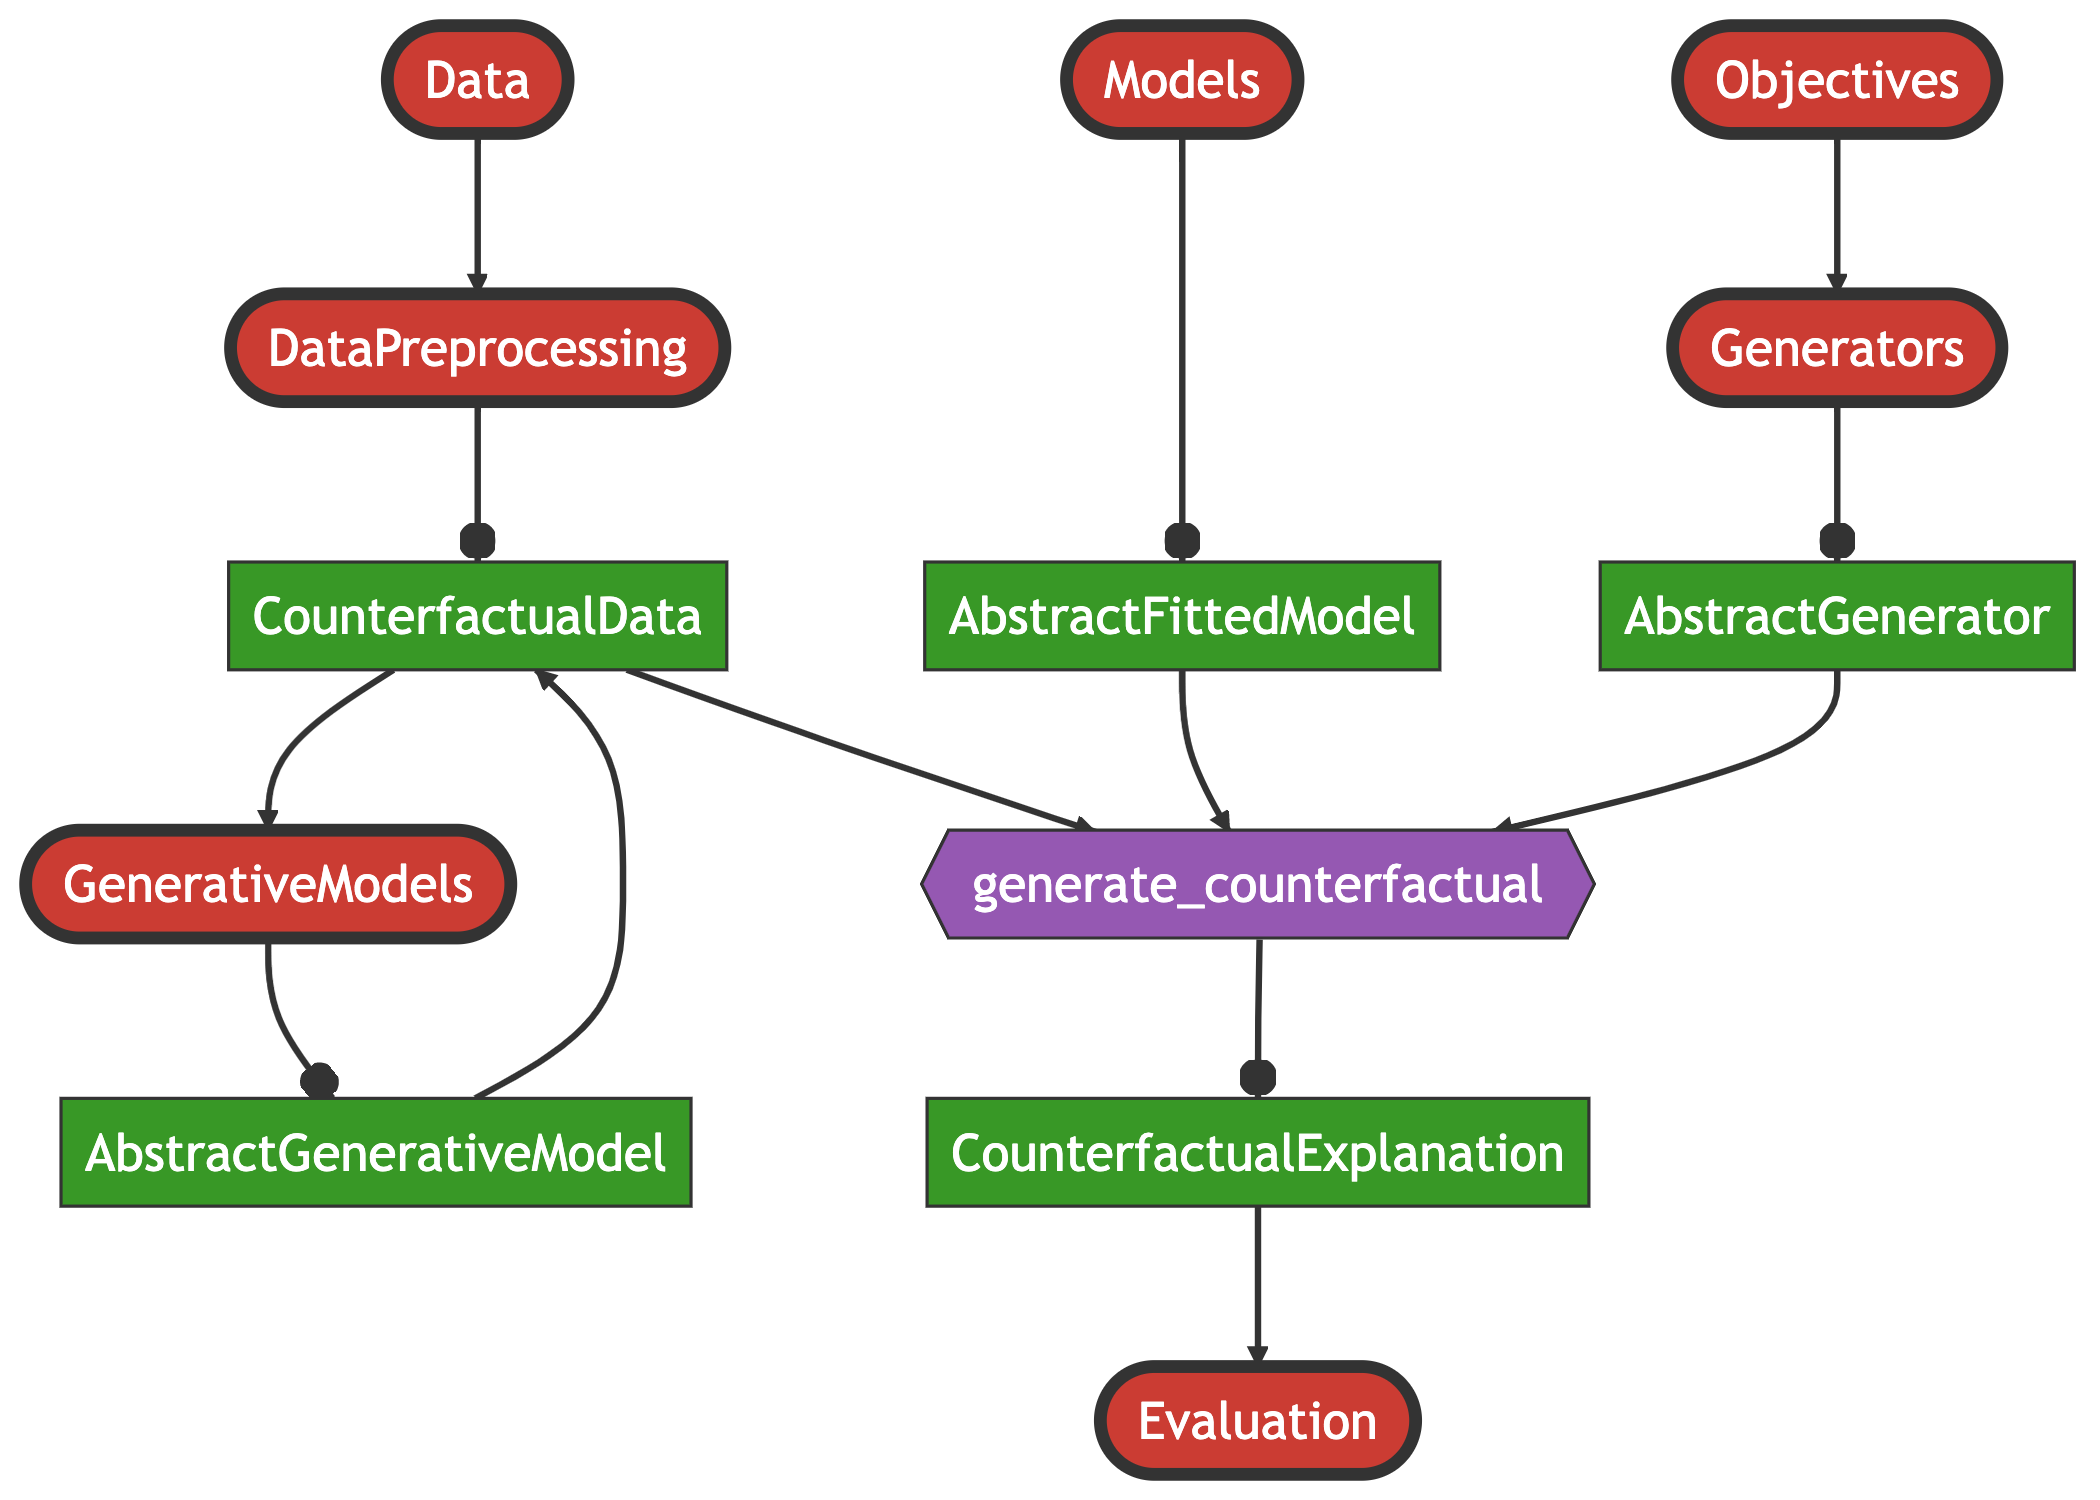
\includegraphics[width=3.33333in,height=2in]{www/pkg_architecture.png}

}

\caption{\label{fig-arch}High-level schematic overview of package
architecture. Modules are shown in red, structs in green and functions
in blue.}

\end{figure}

\hypertarget{sec-use}{%
\section{Basic Usage}\label{sec-use}}

In the following, we begin our exploration of the package functionality
with a simple example. We then turn to a more advanced usage example and
show how users can impose mutability constraints on features.

\hypertarget{a-simple-generic-generator}{%
\subsection{A Simple Generic
Generator}\label{a-simple-generic-generator}}

Listing \ref{lst:simple} below provides a complete example demonstrating
how the framework presented in Section~\ref{sec-method} can be
implemented in Julia with our package. Using a synthetic data set with
linearly separable samples we first define our model and then generate a
counterfactual for a randomly selected sample. Figure~\ref{fig-binary}
shows the resulting counterfactual path in the two-dimensional feature
space. Features go through iterative perturbations until the desired
confidence level is reached as illustrated by the contour in the
background, which indicates the classifier's predicted probability that
the label is equal to 1.

It may help to go through the relevant parts of the code in some more
detail starting from the part involving the model. For illustrative
purposes the \texttt{Models} module ships with a constructor for a
logistic regression model:
\texttt{LogisticModel(W::Matrix,b::AbstractArray)\ \textless{}:\ AbstractFittedModel}.
This constructor does not fit the regression model but rather takes its
underlying parameters as given. In other words, it is generally assumed
that the user has already estimated a model. Based on the provided
estimates two functions are already implemented that compute logits and
probabilities for the model, respectively. Below we will see how users
can use dispatch to extend these functions for use with arbitrary
models. For now, it is enough to note that those methods define how the
model makes its predictions \(M(x)\) and hence they form an integral
part of the counterfactual search. With the model \(M\) defined in the
code below we go on to set up the counterfactual search as follows: 1)
specify the other class as our \texttt{target} label (\(t=1\)) in line
\ref{line:simple-t}; 2) choose a random sample \texttt{x} from the
non-target class in line \ref{line:simple-x}; 3) define the
counterfactual generator in line \ref{line:simple-gen}; and finally run
the counterfactual search in line \ref{line:simple-search}. Generators
like the \texttt{GenericGenerator} take several optional arguments that
govern the strength of the complexity penalty, the step size for
gradient descent and the tolerance for convergence among other things.
This will be discussed in some more detail when looking at the advanced
usage example below.

\begin{lstlisting}[language=Julia, escapechar=@, numbers=left, label={lst:simple}, caption={}] 
# Data and Classifier:
counterfactual_data = load_linearly_separable()
M = fit_model(counterfactual_data, :Linear)

# Factual and Target:
yhat = predict_label(M, counterfactual_data)
target = 2    # target label @\label{line:simple-t}@
candidates = findall(vec(yhat) .!= target)
chosen = rand(candidates)
x = select_factual(counterfactual_data, chosen) @\label{line:simple-x}@

# Counterfactual search:
generator = GenericGenerator() @\label{line:simple-gen}@
ce = generate_counterfactual(
    x, target, counterfactual_data, M, generator) @\label{line:simple-search}@
\end{lstlisting}

\begin{figure}

{\centering 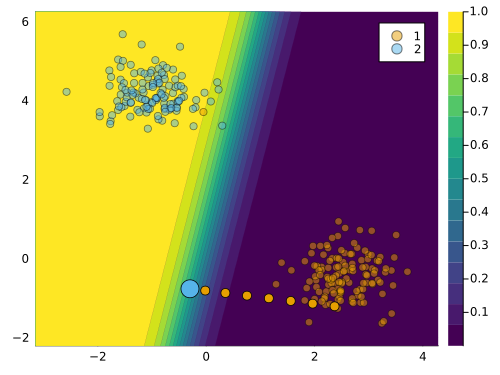
\includegraphics[width=3.33333in,height=2.5in]{www/ce_binary.png}

}

\caption{\label{fig-binary}Counterfactual path using generic
counterfactual generator for conventional binary classifier.}

\end{figure}

In this simple example, the generic generator produces an effective
counterfactual: the decision boundary is crossed (i.e.~the
counterfactual explanation is valid) and upon visual inspection, the
counterfactual seems plausible (Figure~\ref{fig-binary}). Still, the
example also illustrates that things may well go wrong. Since the
underlying model produces high-confidence predictions in regions free of
any data - that is regions with high epistemic uncertainty - it is easy
to think of scenarios that involve valid but unrealistic
counterfactuals. Similarly, any degree of overfitting can be expected to
result in more ambiguous Counterfactual Explanations, since it reduces
the classifier's sensitivity to regions with high aleatoric uncertainty.
Consider, for example, the scenario illustrated in
Figure~\ref{fig-binary-wrong}, which involves the same logistic
classifier, but a massively overfitted version of it. In this case,
generic search may yield an entirely ambiguous counterfactual near the
decision boundary (purple marker) or an unrealistic counterfactual that
has moved well into the target domain, but remains far away from all
other samples (red marker).

\begin{figure}

{\centering 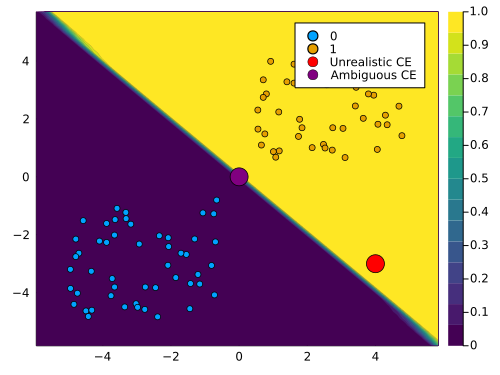
\includegraphics[width=3.33333in,height=2.5in]{www/binary_wrong.png}

}

\caption{\label{fig-binary-wrong}Unrealistic and ambiguous
counterfactuals that may be produced by generic counterfactual search
for an overfitted conventional binary classifier.}

\end{figure}

\hypertarget{more-advanced-generators}{%
\subsection{More Advanced Generators}\label{more-advanced-generators}}

The more advanced generators currently implemented in
\texttt{CounterfactualExplanations.jl} are designed to generate more
realistic counterfactuals. In this context, `realistic' is defined in
the sense that counterfactuals ought to be generated by the same
data-generating process (DGP) that generates the actual data points. To
this end, \textbf{Latent Space} generators like REVISE
\cite{joshi2019realistic} use a separate generative model to learn the
DGP. We refer to them as Latent Space generators, because they search
counterfactuals in the latent embedding learned by the generative
model.\footnote{Currently our implementation relies on a Variational
  Autoencoder (VAE)}. The \textbf{Greedy} approach
\cite{schut2021generating} instead relies on minimizing predictive
uncertainty in order to generate realistic counterfactuals.
\textbf{CLUE} \cite{antoran2020getting} can be thought of as a
combination of these two ideas. The other generator currently
implemented, \textbf{DiCE} \cite{mothilal2020explaining}, generates
multiple counterfactuals at once that are as diverse as possible. This
strategy is based on the intuition that a wide variety of diverse
explanations may be suitable depending on the practical context.

Listing \ref{lst:binary-advanced} below shows a more advanced usage
example involving the DiCE generator. Once again it is worth dwelling on
this for a moment. The \texttt{DiCEGenerator} is instantiated in line
\ref{line:binary-advanced-dice} with a custom Flux optimizer and
decision threshold specified in lines \ref{line:binary-advanced-opt} and
\ref{line:binary-advanced-thresh}, respectively\footnote{Note that all
  differentiable generators except the \texttt{GreedyGenerator} work
  with Flux optimizers and accept them as an optional key argument.}.
The main API call to generate counterfactuals is the same as before, but
note that in line \ref{line:binary-advanced-num} we have specified an
optional key argument that determines how many counterfactuals are
generated. For the DiCE generator it naturally makes sense to generate
multiple counterfactuals, but note that this is in principle also
possible for all other generators.\footnote{By default counterfactuals
  are initialized by adding a small, random perturbation, as this
  improves adversarial robustness \cite{slack2021counterfactual}.
  Therefore, generating multiple counterfactuals will yield multiple
  distinct outcomes even without an explicit diversity constraint.}
Figure~\ref{fig-binary-advanced} shows the resulting output. It was
generated by calling the generic \texttt{plot} method directly on the
object returned by \texttt{generate\_counterfactual}.

\begin{lstlisting}[language=Julia, escapechar=@, numbers=left, label={lst:binary-advanced}, caption={}]
# Generator:
generator = DiCEGenerator( @\label{line:binary-advanced-dice}@
    opt = Flux.Optimise.Descent(0.01), @\label{line:binary-advanced-opt}@
    decision_threshold = 0.7, @\label{line:binary-advanced-thresh}@
    λ = [0.1,5]
)
# Counterfactual search:
counterfactuals = generate_counterfactual(
    x, target, counterfactual_data, M, generator;
    num_counterfactuals=5 @\label{line:binary-advanced-num}@
)
\end{lstlisting}

\begin{figure}

{\centering 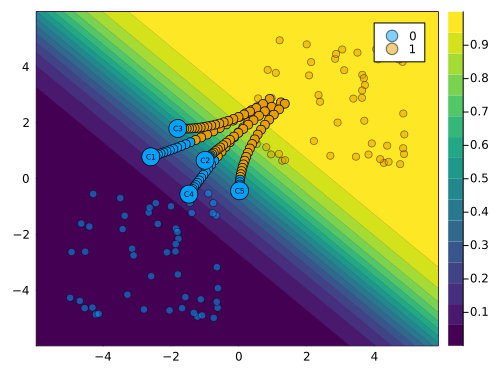
\includegraphics[width=3.33333in,height=2.5in]{www/binary_advanced.png}

}

\caption{\label{fig-binary-advanced}Counterfactual path using the DiCE
generator.}

\end{figure}

\hypertarget{mutability-constraints}{%
\subsection{Mutability Constraints}\label{mutability-constraints}}

In practice, features usually cannot be perturbed arbitrarily. Suppose,
for example, that one of the features used by a bank to predict the
creditworthiness of its clients is \emph{gender}. If a counterfactual
explanation for the prediction model indicates that female clients
should change their gender to improve their creditworthiness, then this
is an interesting insight (it reveals gender bias), but it is not
usually an actionable transformation in practice. In such cases, we may
want to constrain the mutability of features to ensure actionable and
realistic recourse. To illustrate how this can be implemented in
\texttt{CounterfactualExplanations.jl} we will look at the linearly
separable toy dataset again.

Mutability of features can be defined in terms of four different
options: 1) the feature is mutable in both directions, 2) the feature
can only increase (e.g.~\emph{age}), 3) the feature can only decrease
(e.g.~\emph{time left} until your next deadline) and 4) the feature is
not mutable (e.g.~\emph{skin colour}, \emph{ethnicity}, \ldots). To
specify which category a feature belongs to, users can pass a vector of
symbols containing the mutability constraints at the pre-processing
stage. For each feature one can choose from these four options:
\texttt{:both} (mutable in both directions), \texttt{:increase} (only
up), \texttt{:decrease} (only down) and \texttt{:none} (immutable). By
default, \texttt{nothing} is passed to that keyword argument and it is
assumed that all features are mutable in both directions.\footnote{Mutability
  constraints are currently not yet implemented for Latent Space
  generators.}

Below we impose that the second feature is immutable.

\begin{lstlisting}[language=Julia, escapechar=@, numbers=left, label={lst:mutability}, caption={}]
counterfactual_data = CounterfactualData(
    X,ys';mutability=[:both, :none])
\end{lstlisting}

The resulting counterfactual path is shown in
Figure~\ref{fig-mutability} below. Since only the first feature can be
perturbed, the sample can only move along the horizontal axis.

\begin{figure}

{\centering 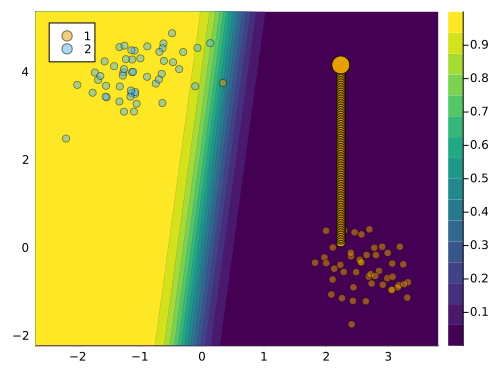
\includegraphics[width=3.33333in,height=2.5in]{www/constraint_mutability.png}

}

\caption{\label{fig-mutability}Counterfactual path with immutable
feature.}

\end{figure}

\hypertarget{sec-custom}{%
\section{Customization and Extensibility}\label{sec-custom}}

One of our priorities has been to make
\texttt{CounterfactualExplanations} customizable and extensible. In the
long term, we aim to add support for more default models and
counterfactual generators. In the short term, it is designed to allow
users to integrate models and generators themselves. Ideally, these
community efforts will facilitate our long-term goals.

\hypertarget{sec-custom-mod}{%
\subsection{Adding Custom Models}\label{sec-custom-mod}}

At the high level, only two steps are necessary to make any supervised
learning model compatible with our package:

\begin{unnumlist}
\item \textbf{Subtyping}: the model needs to be declared as a subtype of \texttt{AbstractFittedModel}.
\item \textbf{Dispatch}: the functions \texttt{logits} and \texttt{probs} need to be extended through custom methods for the model in question.
\end{unnumlist}

To demonstrate how this can be done in practice, we will reiterate here
how native support for \href{https://fluxml.ai/}{\texttt{Flux.jl}}
(\cite{innes2018flux}) deep learning models was enabled.\footnote{Flux
  models are now natively supported by our package and can be
  instantiated by calling \texttt{FluxModel()}.} Once again we use
synthetic data for an illustrative example. Listing \ref{lst:nn} below
builds a simple model architecture that can be used for a multi-class
prediction task. Note how outputs from the final layer are not passed
through a softmax activation function, since the counterfactual loss is
evaluated with respect to logits as we discussed earlier. The model is
trained with dropout for ten training epochs.

\begin{lstlisting}[language=Julia, escapechar=@, numbers=left, label={lst:nn}, caption={}]
n_hidden = 32
output_dim = length(unique(y))
input_dim = 2
model = Chain(
    Dense(input_dim, n_hidden, activation),
    Dropout(0.1),
    Dense(n_hidden, output_dim)
)  
\end{lstlisting}

Listing \ref{lst:mymodel} below implements the two steps that were
necessary to make Flux models compatible with the package. In line
\ref{line:mymodel-subtype} we declare our new struct as a subtype of
\texttt{AbstractDifferentiableModel}, which itself is an abstract
subtype of \texttt{AbstractFittedModel}.\footnote{Note that in line
  \ref{line:mymodel-likelihood} we also provide a field determining the
  likelihood. This is optional and only used internally to determine
  which loss function to use in the counterfactual search. If this field
  is not provided to the model, the loss function needs to be explicitly
  supplied to the generator.} Computing logits amounts to just calling
the model on inputs. Predicted probabilities for labels can then be
computed by passing predicted logits through the softmax function.

\begin{lstlisting}[language=Julia, escapechar=@, numbers=left, label={lst:mymodel}, caption={}]
# Step 1)
struct MyFluxModel <: AbstractDifferentiableModel @\label{line:mymodel-subtype}@
    model::Any
    likelihood::Symbol @\label{line:mymodel-likelihood}@
end

# Step 2)
# import functions in order to extend
import CounterfactualExplanations.Models: logits
import CounterfactualExplanations.Models: probs 
logits(M::MyFluxModel, X::AbstractArray) = M.model(X)
probs(M::MyFluxModel, X::AbstractArray) = softmax(logits(M, X))
M = MyFluxModel(model)
\end{lstlisting}

The API call for actually generating counterfactuals for our new model
is the same as before. Figure~\ref{fig-multi} shows the resulting
counterfactual path for a randomly chosen sample. In this case, the
contour shows the predicted probability that the input is in the target
class (\(t=2\)). Generic search yields a valid, realistic and largely
unambiguous counterfactual.

\begin{figure}

{\centering 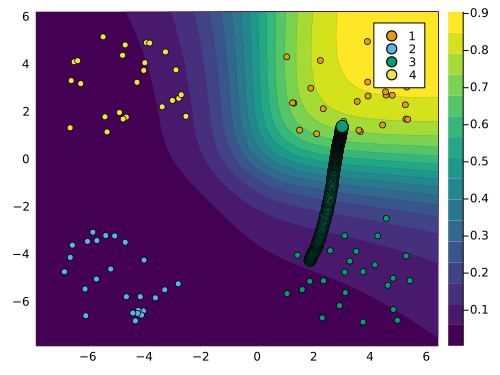
\includegraphics[width=3.33333in,height=2.5in]{www/ce_multi.png}

}

\caption{\label{fig-multi}Counterfactual path using generic
counterfactual generator for multi-class classifier.}

\end{figure}

\hypertarget{sec-custom-gen}{%
\subsection{Adding Custom Generators}\label{sec-custom-gen}}

To illustrate how custom generators can be implemented we will consider
a simple example of a generator that extends the functionality of our
\texttt{GenericGenerator}. We have noted elsewhere that the
effectiveness of Counterfactual Explanations depends to some degree on
the quality of the fitted model. Another, perhaps trivial, thing to note
is that Counterfactual Explanations are not unique: there are
potentially many valid counterfactual paths. One idea building on these
two observations might be to introduce some form of regularization in
the counterfactual search. For example, we could use dropout to randomly
switch features on and off in each iteration. Without dwelling further
on the merit of this idea, we will now briefly show how this can be
implemented.

\hypertarget{a-generator-with-dropout}{%
\subsubsection{A Generator with
Dropout}\label{a-generator-with-dropout}}

Listing \ref{lst:dropout} below implements two important steps: 1)
create an abstract subtype of the
\texttt{AbstractGradientBasedGenerator} and 2) create a constructor
similar to the \texttt{GenericConstructor}, but with one additional
field for the probability of dropout.

\begin{lstlisting}[language=Julia, escapechar=@, numbers=left, label={lst:dropout}, caption={}]
# Abstract suptype:
abstract type AbstractDropoutGenerator <: AbstractGradientBasedGenerator end

# Constructor:
struct DropoutGenerator <: AbstractDropoutGenerator
    loss::Symbol # loss function
    complexity::Function # complexity function
    @$\lambda$@::AbstractFloat # strength of penalty
    decision_threshold::Union{Nothing,AbstractFloat} 
    opt::Any # optimizer
    @$\tau$@::AbstractFloat # tolerance for convergence
    p_dropout::AbstractFloat # dropout rate
end
\end{lstlisting}

Next, in listing \ref{lst:generate} we define how feature perturbations
are generated for our custom dropout generator: in particular, we extend
the relevant function through a method that implements the dropout
logic.

\begin{lstlisting}[language=Julia, escapechar=@, numbers=left, label={lst:generate}, caption={}]
using CounterfactualExplanations.Generators
import Generators: generate_perturbations
import Generators: propose_state
using StatsBase
function generate_perturbations(
    generator::AbstractDropoutGenerator, 
    ce::CouterfactualExplanation
)
    @$s^\prime$@ = deepcopy(ce.@$s^\prime$@)
    new_@$s^\prime$@ = propose_state(
        generator, ce)
    @$\Delta s^\prime$@ = new_@$s^\prime$@ - @$s^\prime$@ # gradient step

    # Dropout:
    set_to_zero = sample(
        1:length(@$\Delta s^\prime$@),
        Int(round(generator.p_dropout*length(@$\Delta s^\prime$@))),
        replace=false
    )
    @$\Delta s^\prime$@[set_to_zero] .= 0
    return @$\Delta s^\prime$@
end
\end{lstlisting}

Finally, we proceed to generate counterfactuals in the same way we
always do. The resulting counterfactual path is shown in
Figure~\ref{fig-dropout}.

\begin{figure}

{\centering 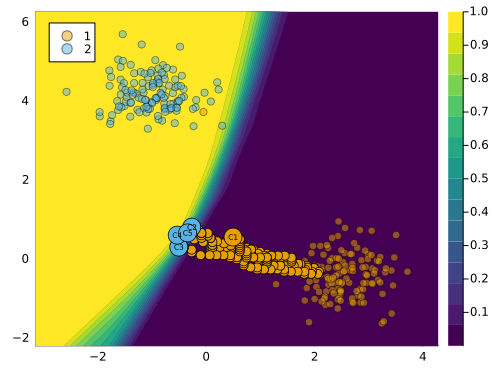
\includegraphics[width=3.33333in,height=2.5in]{www/dropout.png}

}

\caption{\label{fig-dropout}Counterfactual path for a generator with
dropout.}

\end{figure}

\hypertarget{sec-emp}{%
\section{A Real-World Examples}\label{sec-emp}}

Now that we have explained the basic functionality of
\texttt{CounterfactualExplanations.jl} through some synthetic examples,
it is time to work through examples involving real data.

\hypertarget{give-me-some-credit}{%
\subsection{Give Me Some Credit}\label{give-me-some-credit}}

The \textbf{Give Me Some Credit} dataset is one of the tabular
real-world datasets that ship with the package \cite{kaggle2011give}. It
can be used to train a binary classifier to predict whether a borrower
is likely to experience financial difficulties in the next two years. In
particular, we have an output variable
\(y \in \{0=\texttt{no stress},1=\texttt{stress}\}\) and a feature
matrix \(X\) that includes socio-demographic variables like \texttt{age}
and \texttt{income} \(X\). A retail bank might use such a classifier to
determine if potential borrowers should receive credit or not.

For the classification task we use a Multi-Layer Perceptron with dropout
regularization.

Using the generic generator (Wachter) we will generate counterfactuals
for ten randomly chosen individuals that would be denied credit based on
our pre-trained model. With respect to the mutability of features, we
only impose that the \texttt{age} cannot be decreased.

Figure~\ref{fig-credit} shows the resulting counterfactuals proposed by
Wachter in the two-dimensional feature space spanned by the \texttt{age}
and \texttt{income} variables. An increase in income and age is
recommended for the majority of individuals, which seems plausible: both
age and income are typically positively related with creditworthiness.

\begin{figure}

{\centering 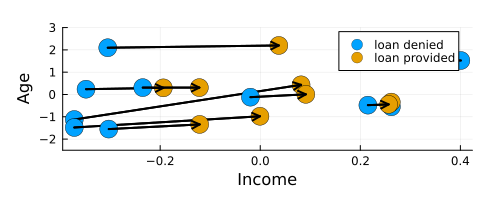
\includegraphics[width=3.33333in,height=2.5in]{www/credit.png}

}

\caption{\label{fig-credit}Give Me Some Credit: counterfactuals for
would-be borrowers proposed by Wachter.}

\end{figure}

\hypertarget{mnist}{%
\subsection{MNIST}\label{mnist}}

For our second example, we will look at image data. The MNIST dataset
contains 60,000 training samples of handwritten digits in the form of
28x28 pixel grey-scale images \cite{lecun1998mnist}. Each image is
associated with a label indicating the digit (0-9) that the image
represents. The data makes for an interesting case study of
Counterfactual Explanations because humans have a good idea of what
realistic counterfactuals of digits look like. For example, if you were
asked to pick up an eraser and turn the digit in
Figure~\ref{fig-mnist-factual} into a four (4) you would know exactly
what to do: just erase the top part. Schut et al.~(2021)
\cite{schut2021generating} leverage this idea to illustrate to the
reader that their methodology produces realistic counterfactuals. In
what follows we replicate some of their findings. You as the reader are
therefore the perfect judge to evaluate the quality of the
Counterfactual Explanations presented below.

On the model side, we will use a simple multi-layer perceptron (MLP).
Listing \ref{lst:mnist-setup} loads the data and the pre-trained MLP. It
also loads a two pre-trained Variational Auto-Encoders, which will be
used by our counterfactual generator of choice for this task: REVISE.

\begin{lstlisting}[language=Julia, escapechar=@, numbers=left, label={lst:mnist-setup}, caption={}]
counterfactual_data = load_mnist()
X, y = unpack_data(counterfactual_data)
input_dim, n_obs = size(counterfactual_data.X)
M = load_mnist_mlp()
vae = load_mnist_vae()
\end{lstlisting}

The proposed counterfactuals are shown in Figure~\ref{fig-mnist}. In the
case in which REVISE has access to an expressive VAE
(Figure~\ref{fig-mnist-strong}), the result looks convincing: the
perturbed image does look like it represents a four (4). In terms of
explainability, we may conclude that removing the top part of the
handwritten nine (9) leads the black-box model to predict that the
perturbed image represents a four (4). We should note, however, that the
quality of counterfactuals produced by REVISE hinges on the performance
of the underlying generative model, as demonstrated by the result on the
right (Figure~\ref{fig-mnist-weak}). In this case, REVISE uses a weak
VAE and the resulting counterfactual is invalid. In light of this, we
recommend using Latent Space search with care.

\begin{figure}

\begin{minipage}[t]{0.33\linewidth}

{\centering 

\raisebox{-\height}{


\includegraphics[width=3.33333in,height=\textheight]{www/mnist_factual.png}

}

}

\subcaption{\label{fig-mnist-factual}Original image.}
\end{minipage}%
%
\begin{minipage}[t]{0.33\linewidth}

{\centering 

\raisebox{-\height}{


\includegraphics[width=3.33333in,height=\textheight]{www/mnist_vae_strong.png}

}

}

\subcaption{\label{fig-mnist-strong}REVISE with expressive VAE.}
\end{minipage}%
%
\begin{minipage}[t]{0.33\linewidth}

{\centering 

\raisebox{-\height}{


\includegraphics[width=3.33333in,height=\textheight]{www/mnist_vae_weak.png}

}

}

\subcaption{\label{fig-mnist-weak}REVISE with weak VAE.}
\end{minipage}%

\caption{\label{fig-mnist}Counterfactual explanations for MNIST using a
Latent Space generator: turning a nine (9) into a four (4).}

\end{figure}

\hypertarget{sec-outlook}{%
\section{Discussion and Outlook}\label{sec-outlook}}

We believe that this package in its current form offers a valuable
contribution to ongoing efforts towards XAI in Julia. That being said,
there is significant scope for future developments, which we briefly
outline in this final section.

\hypertarget{candidate-models-and-generators}{%
\subsection{Candidate models and
generators}\label{candidate-models-and-generators}}

At the time of writing the package supports a handful of default models
and generators either natively or through minimal augmentation. In
future work, we would like to prioritize the addition of further
predictive models and generators. Concerning the former, it would be
useful to add native support for any supervised models built in
\texttt{MLJ.jl}, an extensive Machine Learning framework for Julia
\cite{blaom2020mlj}. This may also involve adding support for regression
models as well as non-differentiable models. In terms of counterfactual
generators, there is list of recent methodologies that we would like to
implement including MINT \cite{karimi2021algorithmic}, ROAR
\cite{upadhyay2021robust} and PROBE
\cite{pawelczyk2022probabilistically}. Through its composable nature,
our package allows for combining different approaches.

\hypertarget{additional-datasets}{%
\subsection{Additional datasets}\label{additional-datasets}}

For benchmarking and testing purposes it will be crucial to add more
datasets to our library. We would like to prioritize datasets that have
typically been used in the literature on counterfactual explanations
including Adult, COMPAS and German Credit \cite{karimi2020survey}. That
being said, there is also scope for adding data sources that have so far
not been explored much in this context including image, audio, natural
language and time-series data.

\hypertarget{sec-dis-foreign}{%
\subsection{Adding Foreign Language Support}\label{sec-dis-foreign}}

The Julia language offers unique support for programming language
interoperability. For example, calling R or Python is made remarkably
easy through auxiliary packages like \texttt{RCall.jl},
\texttt{PythonCall.jl} and \texttt{PyCall.jl}, respectively. Early
experimentation has shown that this functionality can be leveraged to
make \texttt{CounterfactualExplanations.jl} compatible with models that
were developed in foreign programming languages. At the time of writing
this feature is still not mature enough, but we hope to add native
support for explaining \href{https://pytorch.org/}{torch} models trained
in R or Python in the near future.\footnote{Early experiments with this
  feature can be found here:
  \url{https://www.paltmeyer.com/CounterfactualExplanations.jl/dev/tutorials/interop/}}

\hypertarget{sec-conclude}{%
\section{Concluding remarks}\label{sec-conclude}}

The goal of this paper was to illustrate the need for explainability in
machine learning and the promise of Counterfactual Explanations in this
context. To this end, we introduced
\texttt{CounterfactualExplanation.jl}: a package for generating
Counterfactual Explanations and Algorithmic Recourse in Julia. Through
various synthetic and real-world examples, we have demonstrated the
basic usage of the package and shown how it can be easily customized and
extended. We envision this package to one day constitute the go-to place
for explaining arbitrary predictive models through a diverse suite of
counterfactual generators. As a major next step, we would therefore like
to interface our library with the popular
\href{https://alan-turing-institute.github.io/MLJ.jl/dev/}{\texttt{MLJ.jl}}
package for machine learning in Julia. The package can also serve as a
testing ground for new and existing methodological approaches to
Counterfactual Explanations and Algorithmic Recourse. We invite the
Julia community to contribute to these goals through usage, open
challenge and active development.

\hypertarget{sec-ack}{%
\section{Acknowledgements}\label{sec-ack}}

Patrick is grateful to his PhD supervisors and co-authors, Cynthia C. S.
Liem and Arie van Deursen, for being so supportive of his work on
open-source developments. The authors are grateful to the Julia
community for being welcoming and open and for supporting research
contributions like this one.

% **************GENERATED FILE, DO NOT EDIT**************

\bibliographystyle{juliacon}
\bibliography{ref.bib}


\end{document}
